\documentclass[main]{subfiles}

\begin{document}

The calibration mode consists of an acquisition of analog samples, while the rotor 
spins, in order to find compensation parameters for production, mounting and mechanical
non idealities.

To do so, it has been assumed that the sinewaves distortion just creates an ellipse
rotated and not centered at the origin, and that there isn't any higher order 
distortion.
So the algorithm is able to calibrate for an offset, a gain unbalance, and a slightly 
wrong phase shift of the 2 signals.\\

The calibration algorithm can be divided in 2 main blocks:
\begin{itemize}
    \item Identification of ellipse parameters
    \item Unit Circle transform derivation
\end{itemize}

For the ellipse identification, the starting point is the canonical ellipse equation

\begin{equation}
    A x^2 + B xy + C y^2 + D x + E y + F = 0 \label{EQ_ELLIPSE_CANONICAL}
\end{equation}

Where the {\bf$cos$} value has been called {\bf $x$} and the {\bf $sin$} value 
has been called {\bf $y$}

For the identification, the least square method has been chosen, so having acquired
$N$ samples the problem consists of finding the minimum of the quantity

\begin{equation}
    R = \sum_{ii=0}^{N} \left(A x_{ii}^2 + B x_{ii}y_{ii} + C y_{ii}^2 + D x_{ii} + E y_{ii} + F\right)^2
    \label{EQ_LEAST_SQUARES}
\end{equation}

Since the starting equation is in implicit form, the solution is defined only up 
to a multiplicative constant. 
To exclude the trivial solution in which all parameters are zero, and to ensure 
that the problem has a unique solution, the constant parameter was set to 

\begin{equation}
    F = -1
\end{equation}

So (\ref{EQ_LEAST_SQUARES}) becomes

\begin{equation}
    R = \sum_{ii=0}^{N} \left(A x_{ii}^2 + B x_{ii}y_{ii} + C y_{ii}^2 + D x_{ii} + E y_{ii} -1\right)^2
    \label{EQ_LEAST_SQUARES_FORCED}
\end{equation}

To minimize (\ref{EQ_LEAST_SQUARES_FORCED}) partial derivatives have to be zeroed.

\begin{equation}
    \begin{cases}
        \frac{\partial R}{\partial A} = 0\\
        \frac{\partial R}{\partial B} = 0\\
        \frac{\partial R}{\partial C} = 0\\
        \frac{\partial R}{\partial D} = 0\\
        \frac{\partial R}{\partial E} = 0
    \end{cases}
\end{equation}

Doing the math for the first partial derivative you get

\begin{equation}
    \frac{\partial R}{\partial A} = \frac{\partial}{\partial A}\sum_{ii=0}^{N} 
    \left(A x_{ii}^2 + B x_{ii}y_{ii} + C y_{ii}^2 + D x_{ii} + E y_{ii} -1\right)^2
\end{equation}

Exploiting the linearity properties of the problem

\begin{equation}
    \frac{\partial R}{\partial A} = \sum_{ii=0}^{N} \frac{\partial}{\partial A}
    \left(A x_{ii}^2 + B x_{ii}y_{ii} + C y_{ii}^2 + D x_{ii} + E y_{ii} -1\right)^2
\end{equation}

which finally gives

\begin{equation}
    \frac{\partial R}{\partial A} = 2\left[A \sum_{ii=0}^{N} x_{ii}^4 + 
                                           B \sum_{ii=0}^{N} x_{ii}^3y_{ii} + 
                                           C \sum_{ii=0}^{N} x_{ii}^2y_{ii}^2 + 
                                           D \sum_{ii=0}^{N} x_{ii}^3 + 
                                           E \sum_{ii=0}^{N} x_{ii}^2y_{ii} - 
                                             \sum_{ii=0}^{N} x_{ii}^2\right] 
\end{equation}

Since we have to zero the partial derivatives we obtain

\begin{equation}
    A \sum_{ii=0}^{N} x_{ii}^4 + 
    B \sum_{ii=0}^{N} x_{ii}^3y_{ii} + 
    C \sum_{ii=0}^{N} x_{ii}^2y_{ii}^2 + 
    D \sum_{ii=0}^{N} x_{ii}^3 + 
    E \sum_{ii=0}^{N} x_{ii}^2y_{ii}= \sum_{ii=0}^{N} x_{ii}^2
\end{equation}

Repeating this computation for all the partial derivatives we obtain the following 
linear system

\begin{equation} 
    \begin{bmatrix}
        \sum_{ii=0}^{N} x_{ii}^4 & \sum_{ii=0}^{N} x_{ii}^3y_{ii} & \sum_{ii=0}^{N} x_{ii}^2y_{ii}^2 & \sum_{ii=0}^{N} x_{ii}^3 & \sum_{ii=0}^{N} x_{ii}^2y_{ii} \\
        \sum_{ii=0}^{N} x_{ii}^3y_{ii} & \sum_{ii=0}^{N} x_{ii}^2y_{ii}^2 & \sum_{ii=0}^{N} x_{ii}y_{ii}^3 & \sum_{ii=0}^{N} x_{ii}^2y_{ii} & \sum_{ii=0}^{N} x_{ii}y_{ii}^2 \\
        \sum_{ii=0}^{N} x_{ii}^2y_{ii}^2 & \sum_{ii=0}^{N} x_{ii}y_{ii}^3 & \sum_{ii=0}^{N} y_{ii}^4 & \sum_{ii=0}^{N} x_{ii}y_{ii}^2 & \sum_{ii=0}^{N} y_{ii}^3 \\
        \sum_{ii=0}^{N} x_{ii}^3 & \sum_{ii=0}^{N} x_{ii}^2y_{ii} & \sum_{ii=0}^{N} x_{ii}y_{ii}^2 & \sum_{ii=0}^{N} x_{ii}^2 & \sum_{ii=0}^{N} x_{ii}y_{ii} \\
        \sum_{ii=0}^{N} x_{ii}^2y_{ii} & \sum_{ii=0}^{N} x_{ii}y_{ii}^2 & \sum_{ii=0}^{N} y_{ii}^3 & \sum_{ii=0}^{N} x_{ii}y_{ii} & \sum_{ii=0}^{N} y_{ii}^2
    \end{bmatrix}
    \begin{bmatrix}
        A\\
        B\\
        C\\
        D\\
        E
    \end{bmatrix} = 
    \begin{bmatrix}
        \sum_{ii=0}^{N} x_{ii}^2\\
        \sum_{ii=0}^{N} x_{ii}y_{ii}\\
        \sum_{ii=0}^{N} y_{ii}^2\\
        \sum_{ii=0}^{N} x_{ii}\\
        \sum_{ii=0}^{N} y_{ii}
    \end{bmatrix}
    \label{EQ_LIN_SYS_FITTING}
\end{equation}

As it can be seen in (\ref{EQ_LIN_SYS_FITTING}), both the matrix elements and the 
known terms are composed of a sum of some combination of the input samples.

Said that the acquisition could be implemented accumulating samples combinations 
into some accumulators, instead of storing a huge number of samples.

In this case the sampling rate is reduced to $10kHz$, because it is not needed to
go faster and to have more time available for coefficients computing.

The accumulator variables are stored into a structure, shown in listing 
\ref{CODE_ACC_STRUCT}. Here the variables have been defined as 64 bits integers,
in order to stay far from overflow conditions.

\begin{minipage}[h]{\linewidth}
\begin{lstlisting}[caption=Samples accumulator structure, label=CODE_ACC_STRUCT]
    //measures accumulators
    struct {
        int64_t x4;     //x^4
        int64_t x3;     //x^3
        int64_t x2;     //x^2
        int64_t x;      //x

        int64_t y4;     //y^4
        int64_t y3;     //y^3
        int64_t y2;     //y^2
        int64_t y;      //y

        int64_t x3y;    //x^3 * y
        int64_t x2y2;   //x^2 * y^2
        int64_t x2y;    //x^2 * y
        int64_t xy3;    //x * y^3
        int64_t xy2;    //x * y^2
        int64_t xy;     //x * y
    }acc;
\end{lstlisting}
\end{minipage}

In calibration mode, when the ADCs finish their conversion, they trigger an \ac{IRQ}
which is served by an \ac{ISR}, which is different from the one of normal mode.
Here, the samples are just acquired and a constant offset of $2048$ (half the 
range of the ADC) is subtracted, just to avoid having ellipse points passing near 
the origin, breaking the fitting algorithm.
Moving the ellipse to the center also allows to easily count shaft revolutions,
just looking at the samples signs.

The calibration \ac{ISR} starts accumulating the samples after the shaft has done
some electrical revolutions ($10$ at the moment), in order to avoid overflow when 
calibration starts with a still rotor, and so samples have a lot of times the same
value.
With the same logic, the acquisition is stopped when the shaft has completed some 
others electrical revolutions ($100$ at the moment).\\

After having read the ADC registers, the acquisition process consists of the 
computation of a temporary value to be added to the accumulator, the actual sum, 
and finally an overflow check, to avoid calculating parameters with wrong values.
These operation are performed for each accumulator variable.
Listing \ref{CODE_ACC_UPD} shows the operation performed for one of the accumulators.

\begin{minipage}[h]{\linewidth}
\begin{lstlisting}[caption=Samples accumulator update, label=CODE_ACC_UPD]
//---------------------------- x^4 -----------------------------
            
        tmp = (int64_t)adc_data_reg_cos * 
                       adc_data_reg_cos * 
                       adc_data_reg_cos * 
                       adc_data_reg_cos;

        acc_prev = input_calibration_private_vars_v.acc.x4;

        input_calibration_private_vars_v.acc.x4   = tmp + acc_prev;

        if((tmp > 0 && acc_prev > 0 && 
            input_calibration_private_vars_v.acc.x4 < 0) ||
           (tmp < 0 && acc_prev < 0 && 
            input_calibration_private_vars_v.acc.x4 > 0))
        {
            //overflow occurred

            //stop_sampling
            sync_timer_stop();
            //error state
            set_system_status(SYSTEM_STATUS_ERROR);
        }
\end{lstlisting}
\end{minipage}

Finally there are some instructions to count the revolutions of the shaft, shown 
in listing \ref{CODE_TURNS_CNT}.

\begin{minipage}[h]{\linewidth}
\begin{lstlisting}[caption=Turns counter, label=CODE_TURNS_CNT]
//-----------------------------------------------------------------
//                       Find current quadrant
//-----------------------------------------------------------------

    if((adc_data_reg_cos > 0) && (adc_data_reg_sin > 0))
    {
        input_calibration_private_vars_v.quadrant.current = 0;
    }
    if((adc_data_reg_cos < 0) && (adc_data_reg_sin > 0))
    {
        input_calibration_private_vars_v.quadrant.current = 1;
    }
    if((adc_data_reg_cos < 0) && (adc_data_reg_sin < 0))
    {
        input_calibration_private_vars_v.quadrant.current = 2;
    }
    if((adc_data_reg_cos > 0) && (adc_data_reg_sin < 0))
    {
        input_calibration_private_vars_v.quadrant.current = 3;
    }

//-----------------------------------------------------------------
//                            Count turns
//-----------------------------------------------------------------
    if(input_calibration_private_vars_v.quadrant.current == 0 && 
       input_calibration_private_vars_v.quadrant.prev == 3)
    {
        input_calibration_private_vars_v.turns_cnt++;
    }
    else if(input_calibration_private_vars_v.quadrant.current == 3 
            && input_calibration_private_vars_v.quadrant.prev == 0)
    {
        input_calibration_private_vars_v.turns_cnt--;
    }
    input_calibration_private_vars_v.quadrant.prev = 
    input_calibration_private_vars_v.quadrant.current;
\end{lstlisting}
\end{minipage}

After the acquisition is terminated, the main sampling loop is stopped, and the 
system solution is computed inside the main loop.

The solver is a 5 by 5 linear system solver which exploits Gauss Reduction 
Algorithm together with Back Substitution to find the solution of the system.

Gauss Reduction converts a system in the form
\begin{equation}
    \begin{bmatrix}
        a_{00} & a_{01} & a_{02}\\
        a_{10} & a_{11} & a_{12}\\
        a_{20} & a_{21} & a_{22}
    \end{bmatrix}
    \begin{bmatrix}
        x_0\\
        x_1\\
        x_2
    \end{bmatrix}=
    \begin{bmatrix}
        b_0\\
        b_1\\
        b_2
    \end{bmatrix}
\end{equation}

to the form 

\begin{equation}
    \begin{bmatrix}
        a_{00} & a_{01} & a_{02}\\
        0 & a'_{11} & a'_{12}\\
        0 & 0 & a'_{22}
    \end{bmatrix}
    \begin{bmatrix}
        x_0\\
        x_1\\
        x_2
    \end{bmatrix}=
    \begin{bmatrix}
        b_0\\
        b'_1\\
        b'_2
    \end{bmatrix}
\end{equation}

So that the last variable can be simply obtained as

\begin{equation}
    x_2 = \frac{b'_2}{a'_{22}}
\end{equation}

After that, you can go back to upper rows substituting already computed solutions 
to solve for other variables.

During both Gauss Reduction and Back Substitution, it is essential to avoid 
divisions by zero.
In particular, it may happen that one element on the main diagonal of the reduced
matrix is null. If it is the case, the matrix is singular and the system hasn't a 
well defined solution.

Moreover, before applying Gauss Reduction, the matrix rows are sorted in order to 
have always the greater possible divisor during Gauss reduction.
So at the first iteration, the row with greater first element is brought at first 
place; at second iteration the row with greater second element among the remaining 
ones is placed as second row; and so on.

In listing \ref{CODE_ROW_SORT} it is shown the sorting function, while in listing 
\ref{CODE_GAUSS} it is reported the Gauss Reduction implementation, and in 
listing \ref{CODE_BACK_SUBS} there is the Back substitution.

\begin{minipage}[h]{\linewidth}
\begin{lstlisting}[caption=Row sorting, label=CODE_ROW_SORT]
/**
 * @brief Sorts matrix rows looking at elements on the main diagonal
 *        (Upper rows have the greater diagonal term in that position)
 * @param _matrix5      matrix of equations coefficients
 * @param _known_terms  array of equations known terms
 * @return
 */
void sort_rows(float _matrix5[LIN_SYS_SIZE][LIN_SYS_SIZE], 
                float* _known_terms)
{
    uint8_t ii, jj;
    uint8_t index_max;
    
    //loop on rows
    for(ii = 0; ii < LIN_SYS_SIZE; ii++)
    {
        //find maximum element at ii column
        index_max = ii;
        for(jj = ii; jj < LIN_SYS_SIZE; jj++)
        {
            if(ABS(_matrix5[jj][ii]) > 
               ABS(_matrix5[index_max][ii]))
            {
                index_max = jj;
            }
        }

        //swap row ii with row index_max
        swap_rows(_matrix5[ii], _matrix5[index_max], 
                  &_known_terms[ii], 
                  &_known_terms[index_max]);
    }

    return;
}
\end{lstlisting}
\end{minipage}

\begin{minipage}[h]{\linewidth}
\begin{lstlisting}[caption=Gauss Reduction Implementation, label=CODE_GAUSS]
/**
 * @brief Reduces a matrix to staircase pattern using Gauss algorithm
 * @param _matrix5      matrix
 * @param _known_terms  known terms array
 * @return Reduction result: Reduction OK (1) / Singular Matrix (0)
 */
uint8_t gauss_reduction(float _matrix5[LIN_SYS_SIZE][LIN_SYS_SIZE], 
                        float* _known_terms)
{
    uint8_t retVal = 1;
    uint8_t ii,jj;
    uint8_t kk;
    float coeff;

    //loop on rows (not last one)
    for(jj = 0; jj < (LIN_SYS_SIZE-1); jj++)
    {
        //loop on following rows
        for(ii = jj + 1; ii < LIN_SYS_SIZE; ii++)
        {
            //avoid 0 division
            if(0.0f != _matrix5[jj][jj])
            {
                //calculate scaling for jj row to 
                //zero the element [ii][jj]
                coeff = _matrix5[ii][jj] / _matrix5[jj][jj];

                //subtract scaled row jj to row ii element by element
                for(kk = 0; kk < LIN_SYS_SIZE; kk++)
                {
                    _matrix5[ii][kk] -= coeff * _matrix5[jj][kk];
                }

                _known_terms[ii] -= coeff * _known_terms[jj];
            }
            else 
            {
                //if zero division --> singular matrix
                retVal = 0;
            }
        }
    }
    return retVal;
}
\end{lstlisting}
\end{minipage}

\begin{minipage}[h]{\linewidth}
\begin{lstlisting}[caption=Back Substitution Implementation, label=CODE_BACK_SUBS]
/**
 * @brief Calculate solutions with back substitution after 
 *        Gauss reduction
 * @param _matrix5      matrix
 * @param _known_terms  known_terms array
 * @param _solutions    array to store solutions
 * @return Substitution result: Substitution OK (1)
                                Singular Matrix (0)
 */
uint8_t back_substitution(float _matrix5[LIN_SYS_SIZE][LIN_SYS_SIZE], 
                          float* _known_terms, float* _solutions)
{
    int8_t ii,jj;
    uint8_t retVal = 1;

    //loop rows from last one to first one
    for(ii = LIN_SYS_SIZE-1; ii >= 0; ii--)
    {
        //the solution is calculated combining the known term 
        //with the already calculated solutions
        _solutions[ii] = _known_terms[ii];
        for(jj = LIN_SYS_SIZE-1; jj > ii; jj--)
        {
            _solutions[ii] -= _solutions[jj] * _matrix5[ii][jj];
        }

        //avoid division by 0
        if(0.0f != _matrix5[ii][ii])
        {
            _solutions[ii] /= _matrix5[ii][ii];
        }
        else 
        {
            //if the diagonal element is zero valued, 
            //the matrix is non-inveritble system has 
            //no single solution
            retVal = 0;
        }
    }
    return retVal;
}
\end{lstlisting}
\end{minipage}

\begin{figure}[h]
    \centering
    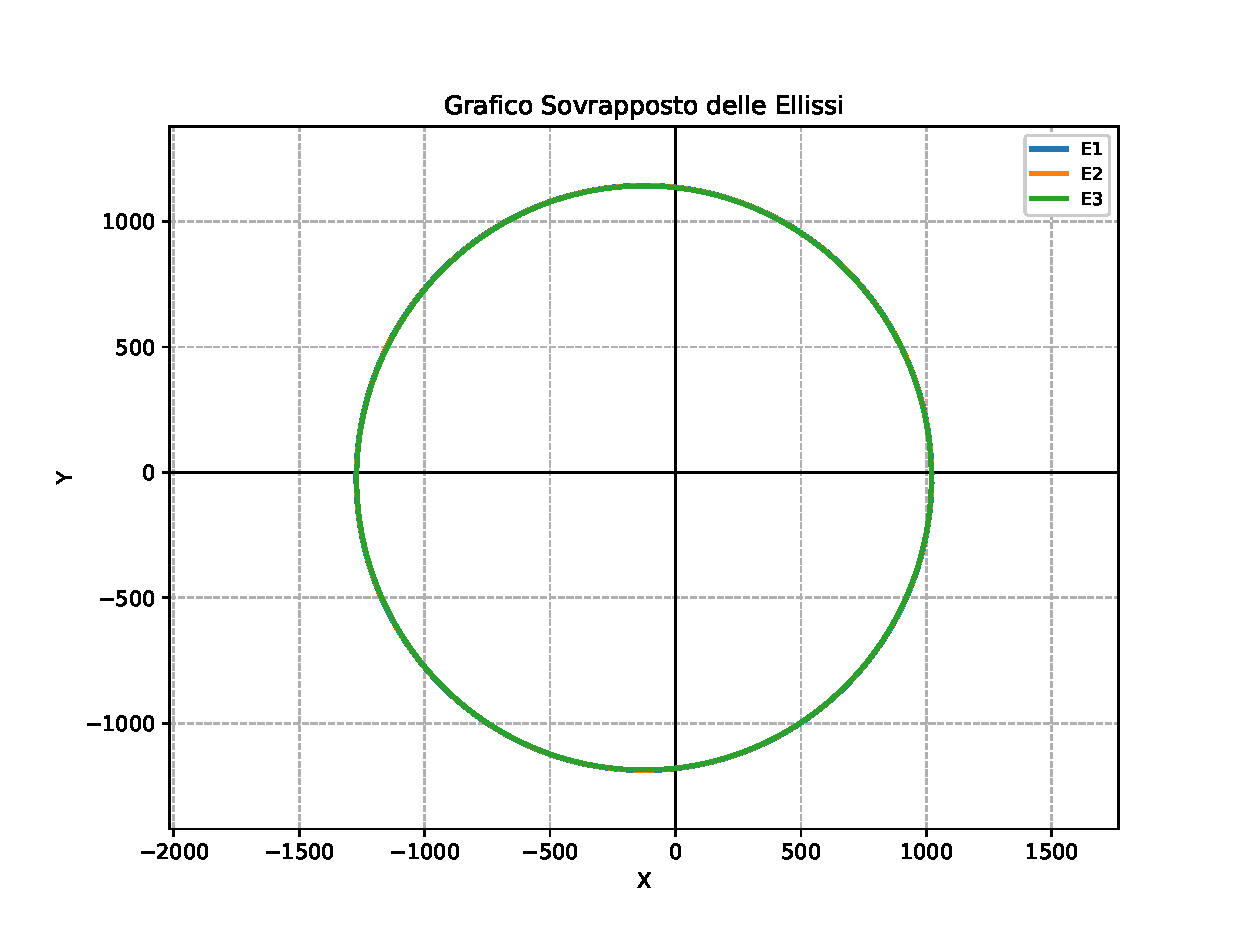
\includegraphics[width=0.7\linewidth]{img/ellipse_fitting_plot.eps}
    \caption{Overlapping of 3 subsequent ellipse fittings}
    \label{FIG_ELL_PLOT}
\end{figure}

Figure \ref{FIG_ELL_PLOT} shows the results of three subsequent ellipse fitting
calculations, overlapped on the same graph.
As it can be seen, the three results are exactly one on top of the other, and
the computation can be considered repeatable enough to perform a calibration.
The amplitude of the ellipse is given in ADC counts and as you can see, it 
covers quite well the 12 bit full scale range.\\

After having obtained the ellipse equation parameters, to complete the calibration, 
the unit circle transformation matrix has to be computed.

That transformation will be defined with 2 offsets, one for cos and one for sin,
and a transformation matrix to compensate for scaling and rotation.

\end{document}